\section{Results and analysis}\label{sec:Results}
\begin{figure}[h!]
\begin{tikzpicture}[node distance = 1cm]
\node (MOS) [rectangle,rounded corners,draw, align=center]{Maximal Overlap\\ Split\\1159479 fragments};
\node (MOF) [right = of MOS, rectangle,rounded corners,draw, align=center]{Maximal Overlap\\ Full\\1160117 fragments};
\node (SDS) [below right= 1 cm and -1 cm of MOS, rectangle,rounded corners,draw, align=center]{Shortest Derivation\\ Split\\491533 fragments};
\draw[dashed](MOS)--(MOF)--(SDS)--(MOS);
\end{tikzpicture}
\caption{The grammars and their size}
\label{f:grammars}
\end{figure}
%SIZE OF THE GRAMMARs

Figure \ref{f:grammars} summarizes the three grammars we investigate.
%There are three grammars we analyze: maximal overlap extraction with both split and full estimation, and shortest derivation with split estimation.
The split estimation was done by interpolating the estimates produced by ten random (equal) splits.  All grammars have been smoothed with PCFG rules to maximize coverage. In the maximal overlap approach, this is done internally as defined in \ddop{}. In the shortest derivation apporach, we redistribute a proportion $p_{unkn}$ of the probability mass over the PCFG grammar. $p_{unkn}$ was found to be $1.41\times 10^{-3}$ for our dataset.%0.00140590480016

%Iets over tijd?
%	Het koste slechts 45 uur met 2 servers:
%	$ time sh batch.sh wsj-02-21.mrg 39833 1 5
%	$ time sh batch.sh wsj-02-21.mrg 39833 6 10
%	[...]
%	2490344.51user 2819.26system 44:37:59elapsed 1551%CPU (0avgtext+0avgdata23866400maxresident)k
%	32056inputs+1353048outputs (13major+375643658minor)pagefaults 0swaps

\subsection{Parsing performance}

\begin{table*}
\center
%
%\begin{tabular}{l | ccc}
%&Maximal~Overlap&Maximal~Overlap&Shortest~Derivation\\
%&Full& Split&Split\\\hline
%labeled recall&		90,97&	90.14&	84.90\\
%labeled precision&		90.25&	90.10&	84.39\\
%labeled f-measure&		90.61&	90.12&	84.64\\
%exact match&		53.27&	49.53&	39.25\\
%\end{tabular}
%
%\caption{Results for 321 sentences of length$\leq 15$}
%


\begin{tabular}{l | ccc}
&Maximal~Overlap&Maximal~Overlap&Shortest~Derivation\\
& Full& Split&Split\\\hline
labeled recall&		86.17&	85.11&	79.20\\
labeled precision&		86.05&	85.50&	79.32\\
labeled f-measure&		86.11&	85.31&	79.26\\
exact match&		28.32&	25.87&	16.52\\
\end{tabular}

\caption{Results for 1229 sentences of length$\leq 40$}


\label{t:performance}
\end{table*}

Table \ref{t:performance} shows the parsing performance for the three grammars we constructed. Note that the POS-tags were passed to the parser in all cases, so tagging accuracy was 100\% and is omitted from this table. 
Note that we did only one run on a predefined train/ test split.

Both Maximal Overlap grammars perform much better than the Shortest Derivation one, in spite of the latter being consistent. 
This might well be related to the size of the grammars: the Shortest Derivation grammar has less than half the number of fragments the other two grammars have. 

A second explanation might be the smoothing we conducted. Recall that the coverage of the Maximal Overlap approach is catered in a rather natural way, by extending the symbolic grammar with all PCFG rules from the treebank and treating them like the other fragments in the estimation. In the case of Shortest Derivation however, the coverage was a bit more artificial. $p_{unkn}$ was computed over all folds and used to redistribute weights over a classical PCFG constructed from the entire treebank. 


Furthermore, we observe that the performance of Maximal Overlap with Full estimation performs slightly better than the Split estimation. The latter was expected to prevent overfitting, but apparently was not helpful in this case. As the weights of these two grammars do not diverge much, it would be recommended to do several runs (with different splits for train and test set). This was however not feasible for us, given the limited amount of time for this project.


\subsection{Pairwise comparison of the grammars}
In each plot, two grammars are compared to each other. The fragments are presented in a scatter plot, with the weights assigned by the two grammars along the axes. The weights are best visualized on a logarithmic scale. However, it is also informative to see those fragments with value zero. Therefore, the first interval ($[0,10^{-6}]$) is linear, while the rest of the plot is logarithmic. 
The difference between grammars is represented by the distance of the points to the \emph{identity line} $x=y$.
The color corresponds to some feature, e.g. the depth of the fragment. The color mapping is also logarithmic. 

% 1 figuur:
% SDS MOS depth (both split)
% SDS MOF depth (original DDOP en DOP*)
% MOS MOF depth (split vs full)
\begin{figure*}
\center
\begin{subfigure}{0.32\textwidth}
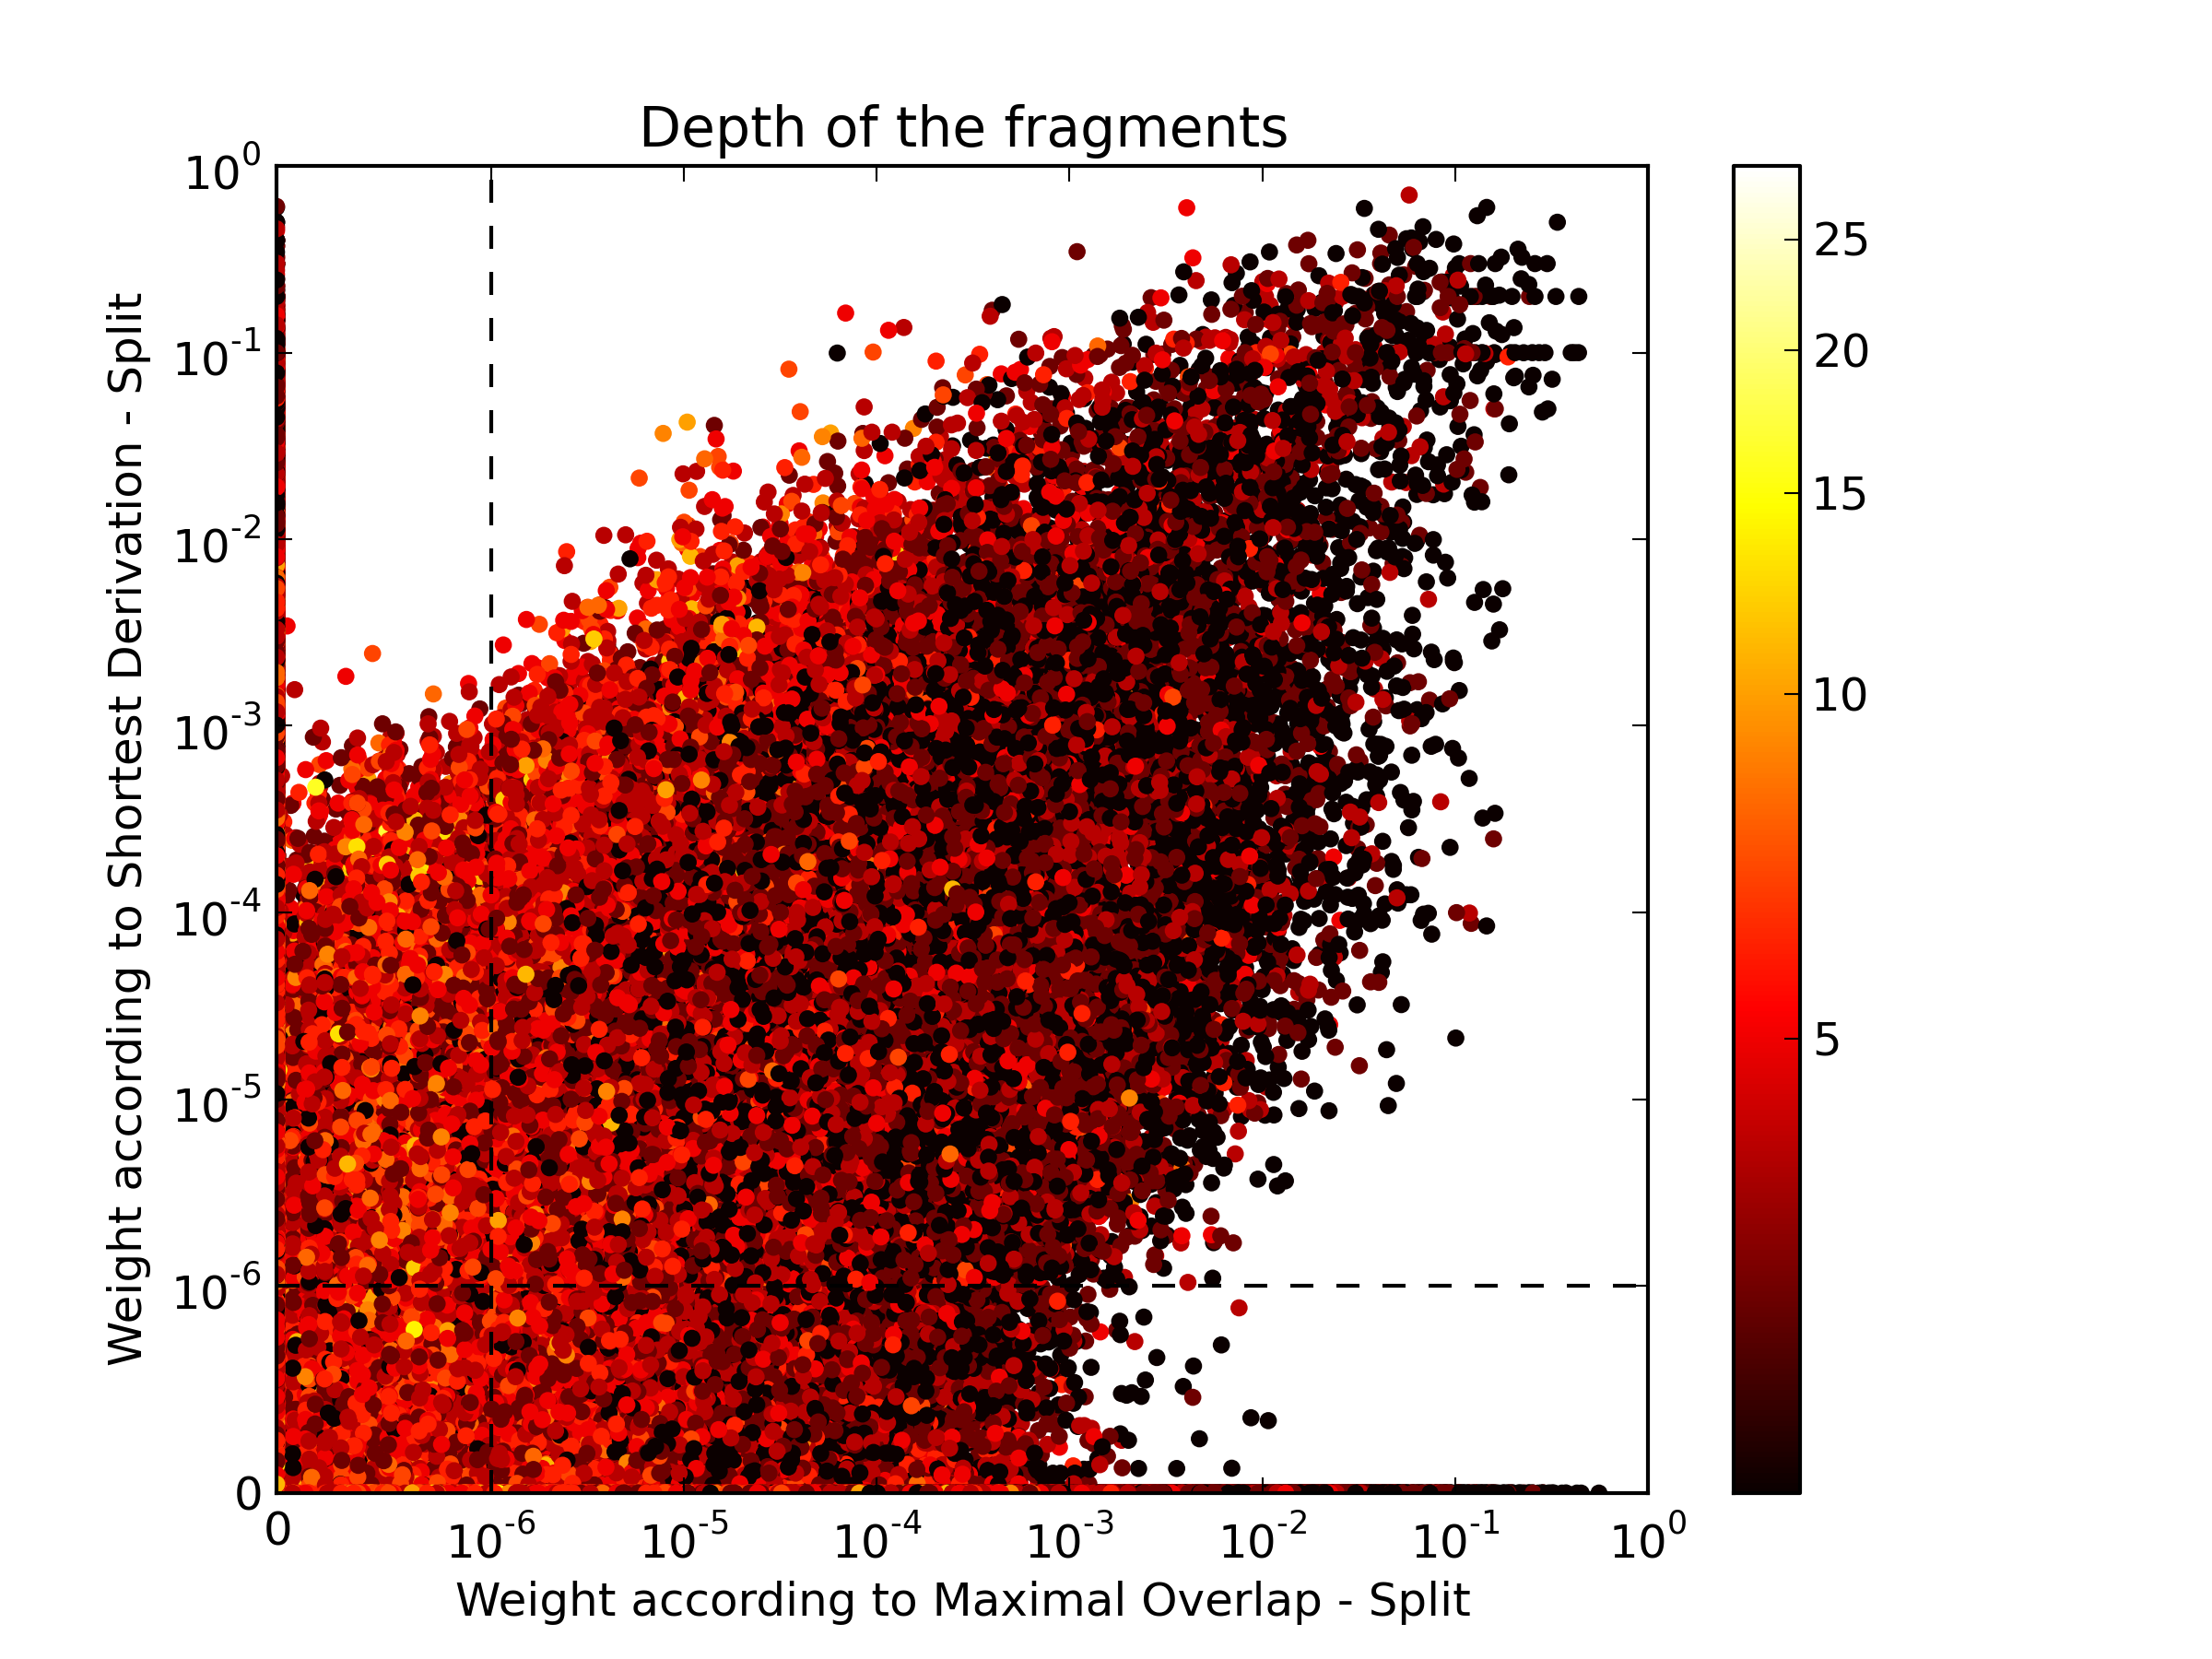
\includegraphics[width=\linewidth,trim=0.5cm 0cm 2.5cm 0.5cm, clip=true]{../data/plots/0.png}
\caption{}
\label{f:SDS-MOS}
\end{subfigure}
\begin{subfigure}{0.32\textwidth}
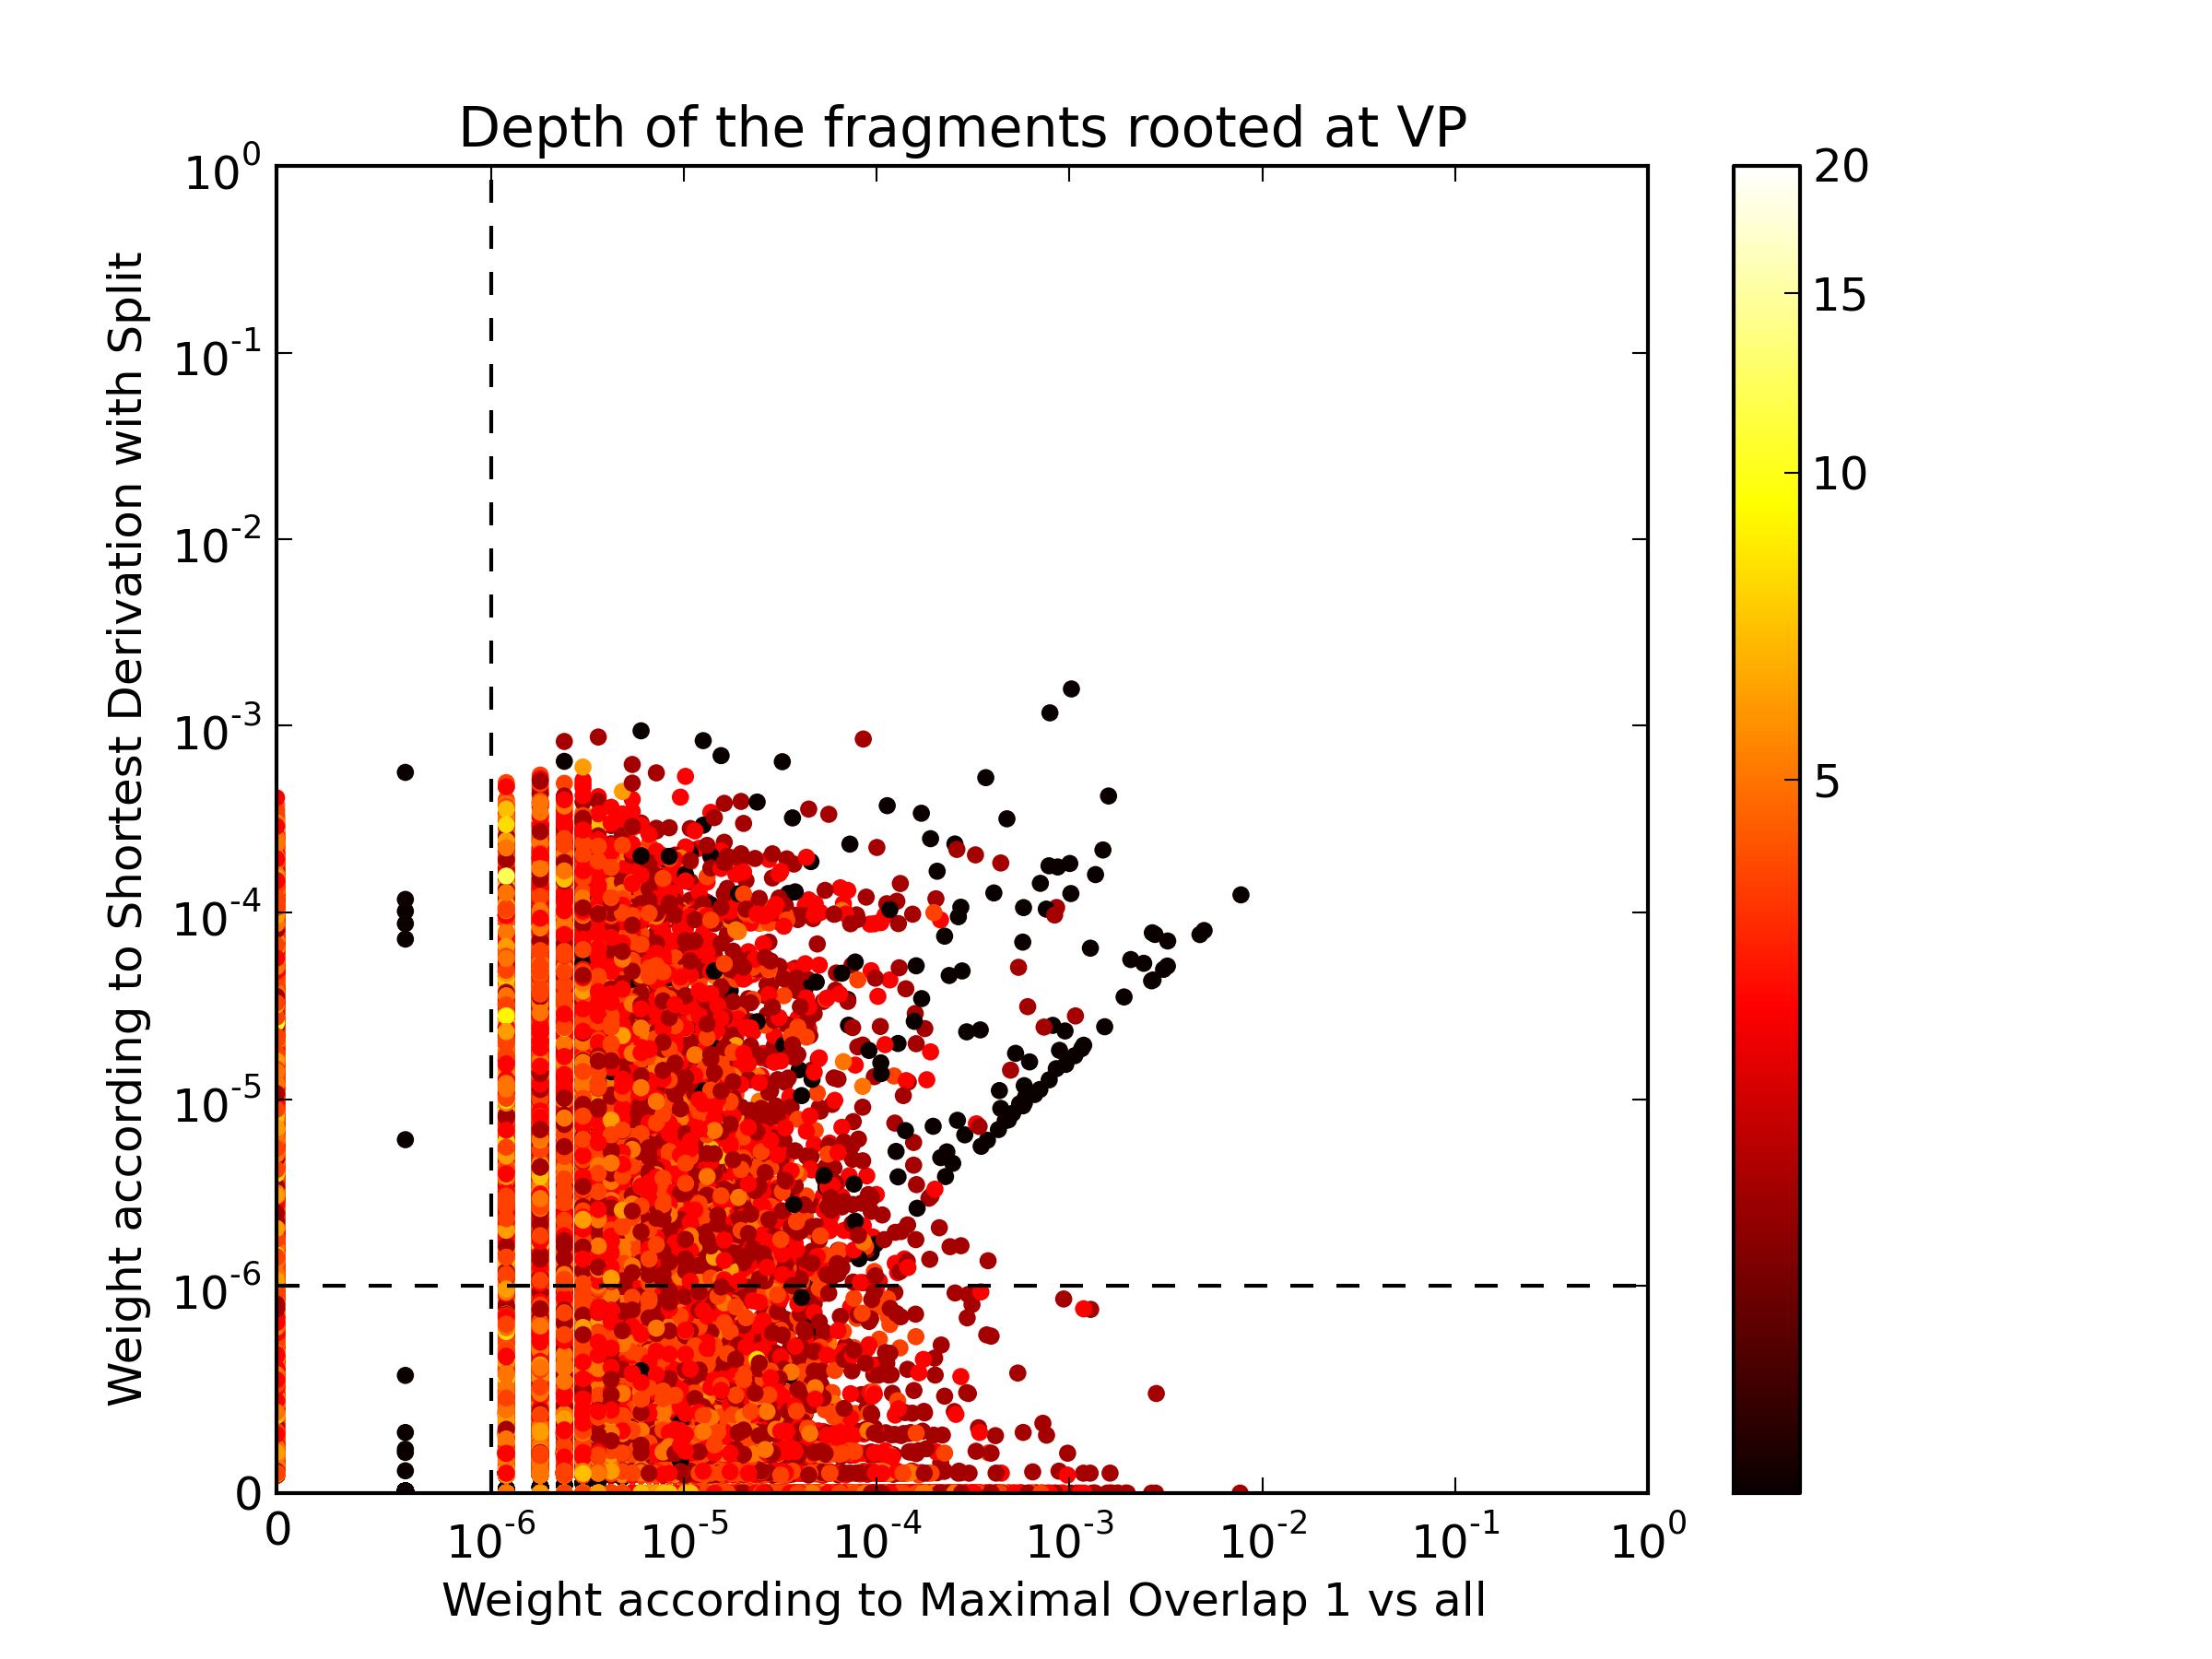
\includegraphics[width=\linewidth,trim=0.5cm 0cm 2.5cm 0.5cm, clip=true]{../data/plots/1.png}
\caption{}
\label{f:SDS-MOF}
\end{subfigure}
\begin{subfigure}{0.32\textwidth}
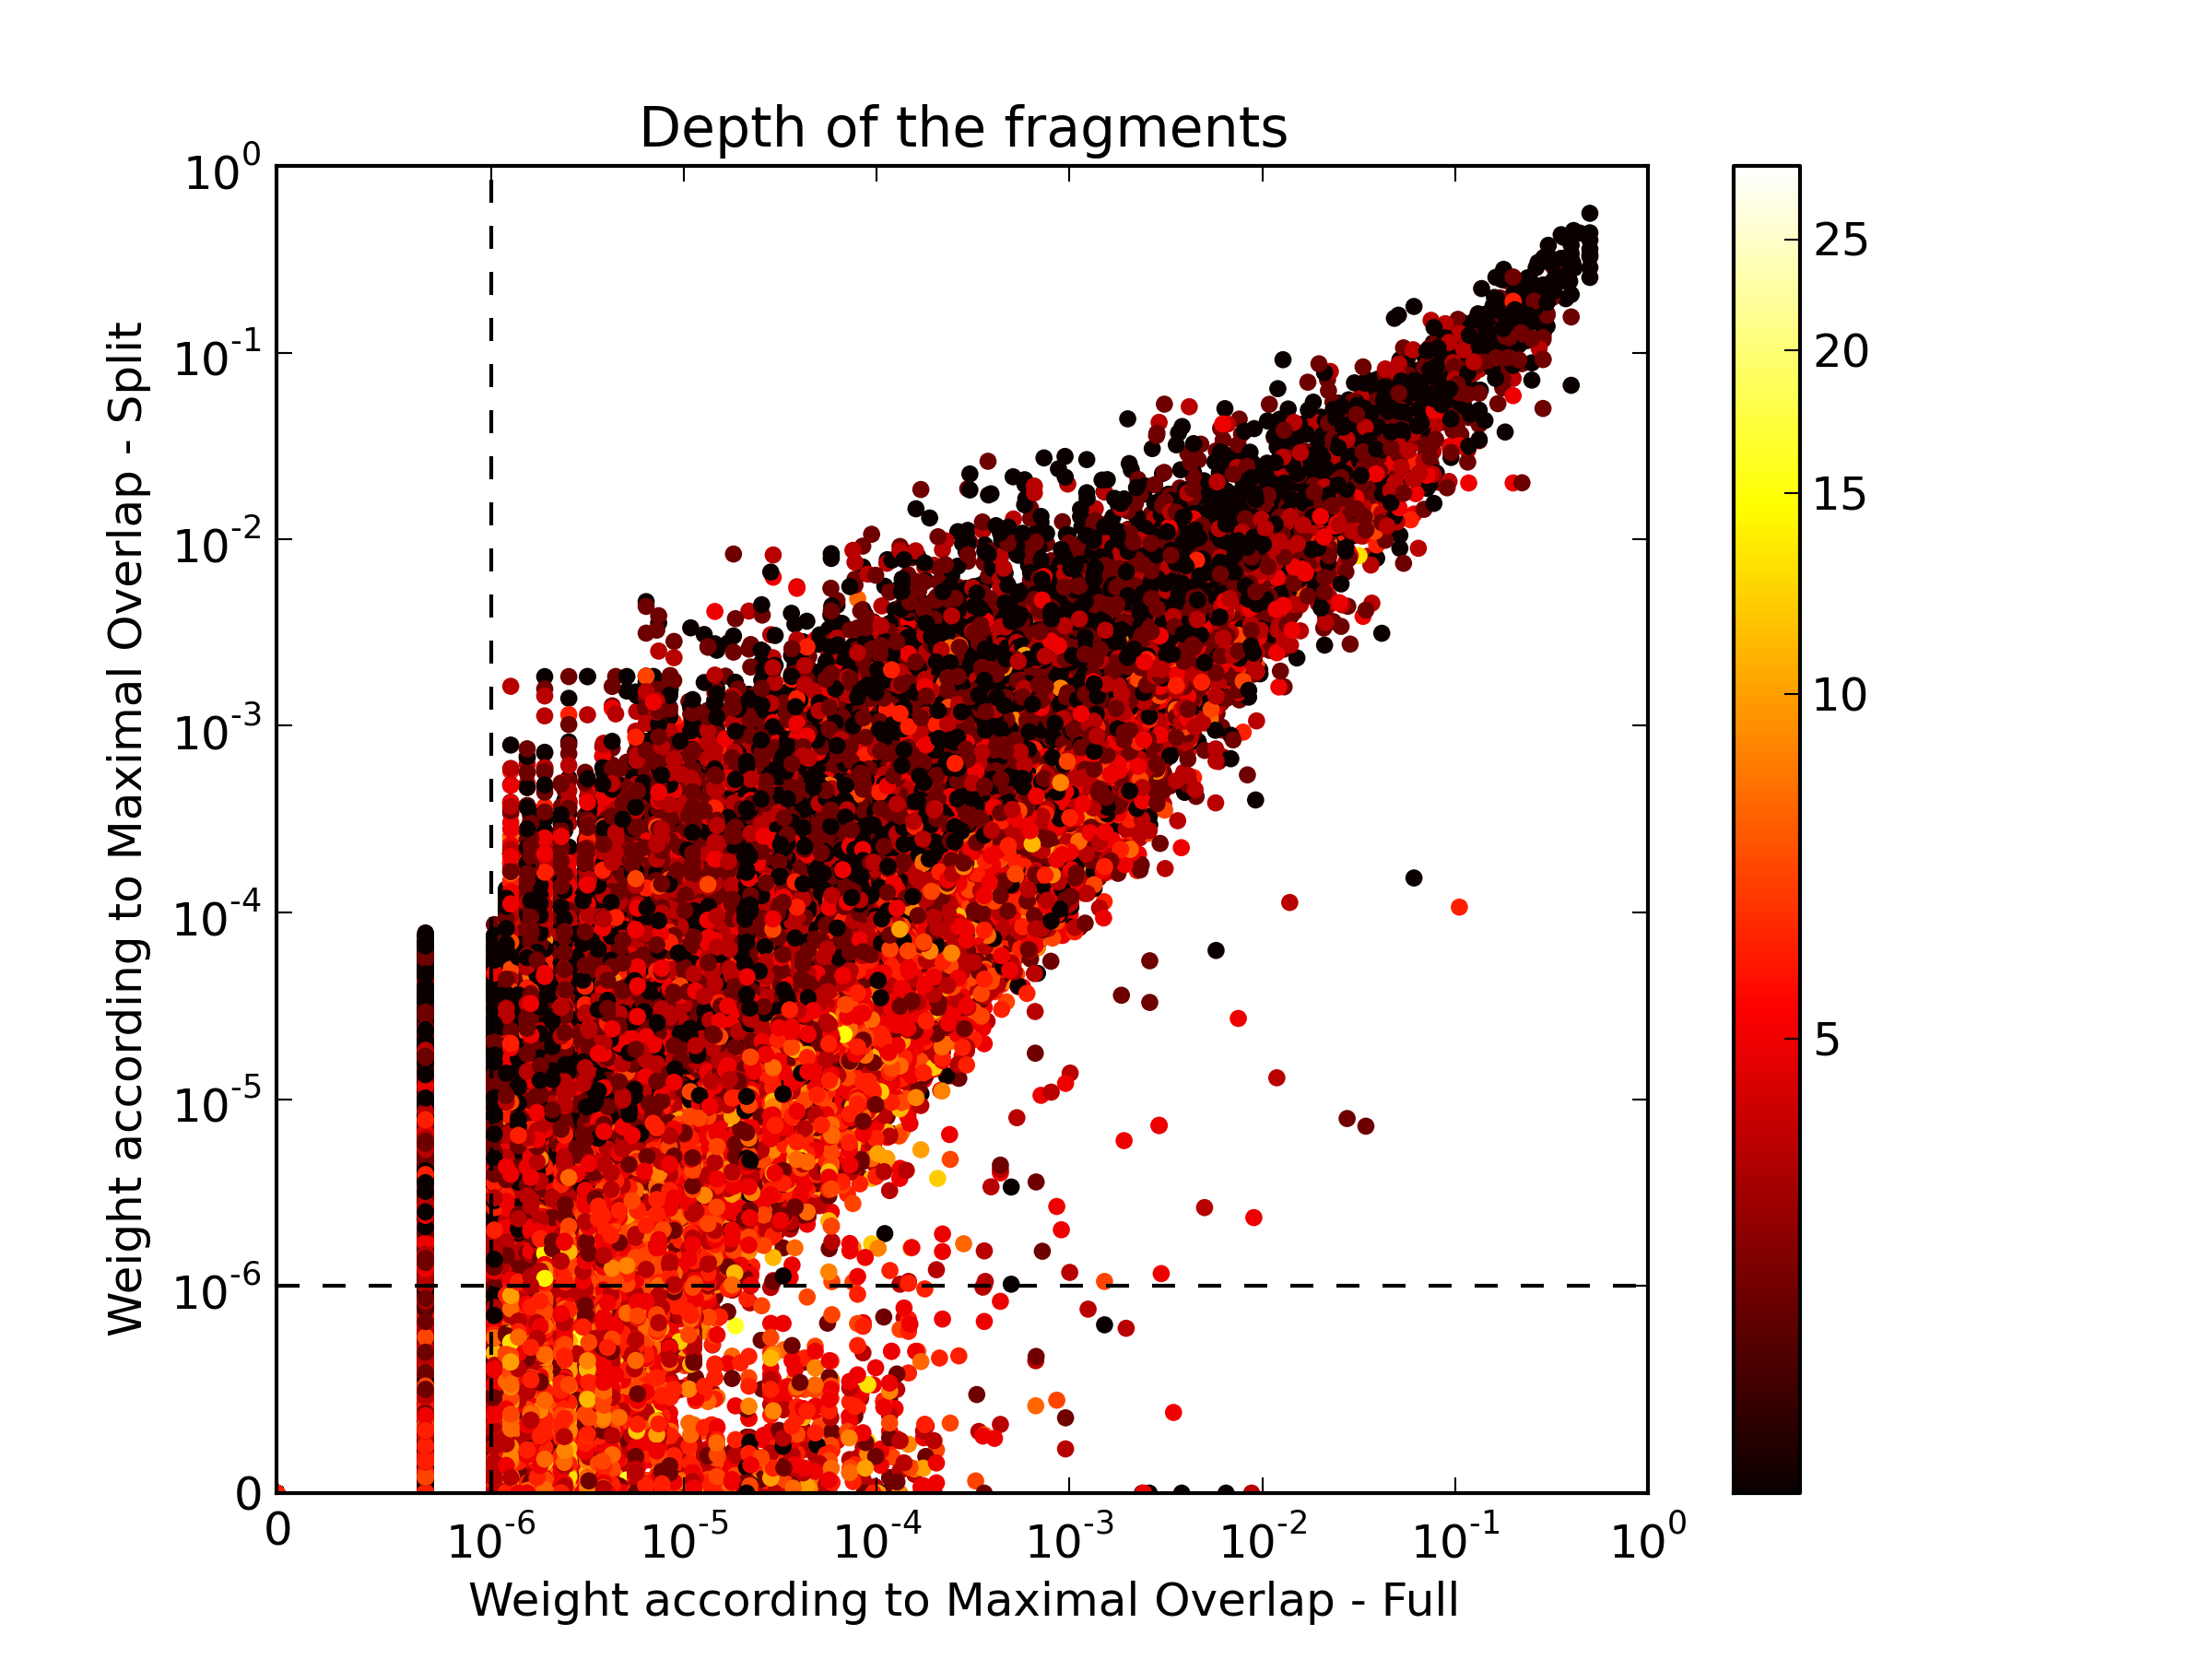
\includegraphics[width=\linewidth,trim=0.5cm 0cm 2.5cm 0.5cm, clip=true]{../data/plots/2.png}
\caption{}
\label{f:MOS-MOF}
\end{subfigure}

\caption{Comparing three grammars by depth of the fragments}
\label{f:depth3}
\end{figure*}

\paragraph{Depth of the fragments}
In figure \ref{f:depth3}, the color of the points in the scatter plot refer to the depth of the fragments. Depth is a common measure of fragment size. Johnson shows in \shortcite{johnson2002} that the original DOP1 had a bias towards larger fragments. 

Plot \ref{f:MOS-MOF} illustrates the effect of the split estimation as compared to full estimation. We see a remarkable, almost linear separation of fragments with larger depth (lighter color) below the identity line, and fragments with smaller depth above it. This indicates that the split estimation tends to reduce the bias towards larger fragments.

In plots \ref{f:SDS-MOS} and \ref{f:SDS-MOF}, the shortest derivation extraction is compared to both maximal overlap grammars. Although the correlation between weight assignment and depth is less evident, the area above the identity line gets fragments with a lighter color. This reveal that shortest derivation extraction gives a higher weight to large fragments than maximal overlap. 


\paragraph{Width of the fragments}

The width of the fragments is another measure of their size. It is defined as the number of substitution sites plus the number of terminals.As an example, in figure \ref{f:width1a} both extraction methods are compared with split estimation.  The dark peak on the right corresponds to the smoothing: PCFG fragments have low width by definition. In figure \ref{f:width1b} only fragments of depth 2 and deeper are shown, and the dark peak is gone.

The way the fragments with certain width are distributed does not differ much from the depth, of course width and depth are strongly correlated themselves. We have also looked at the number of substitution sites and the number of terminals of isolation, but this did not reveal much more than the total width. 



\begin{figure*}
\center
\begin{subfigure}{0.45\textwidth}
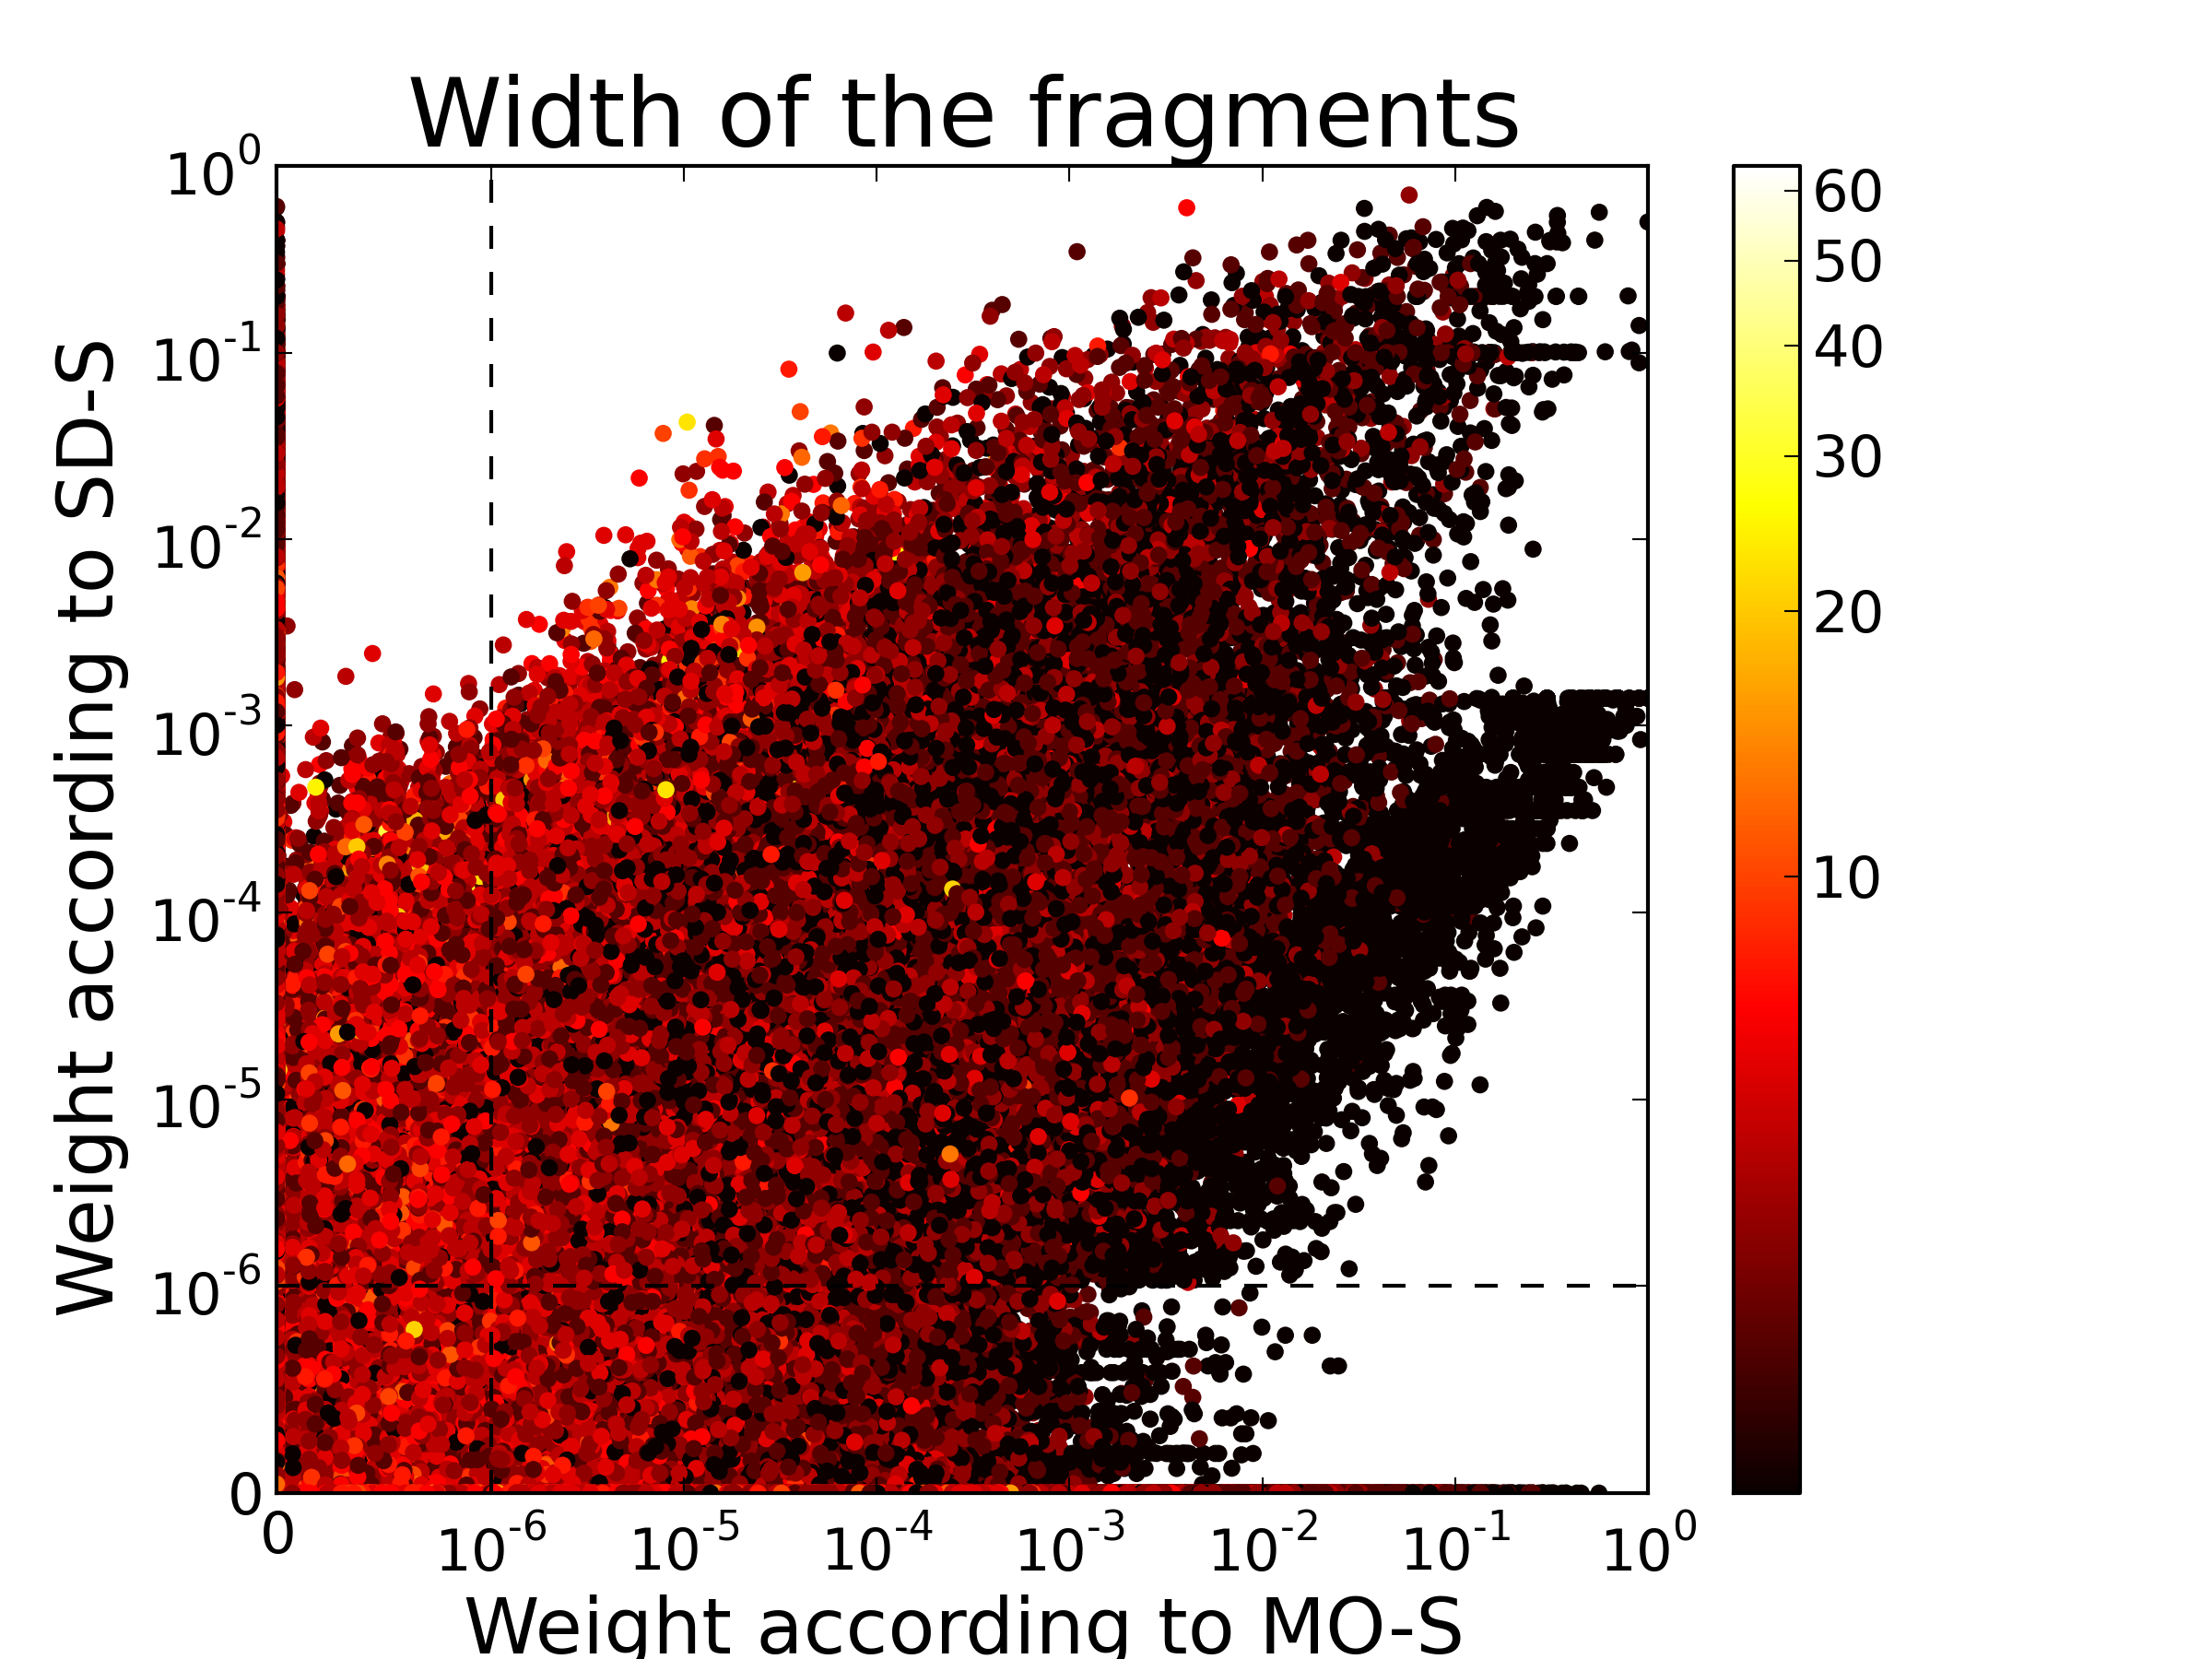
\includegraphics[width=\linewidth,trim=0.5cm 0cm 2.5cm 0.5cm, clip=true]{../data/plots/6.png}
\caption{}
\label{f:width1a}
\end{subfigure}
\begin{subfigure}{0.45\textwidth}
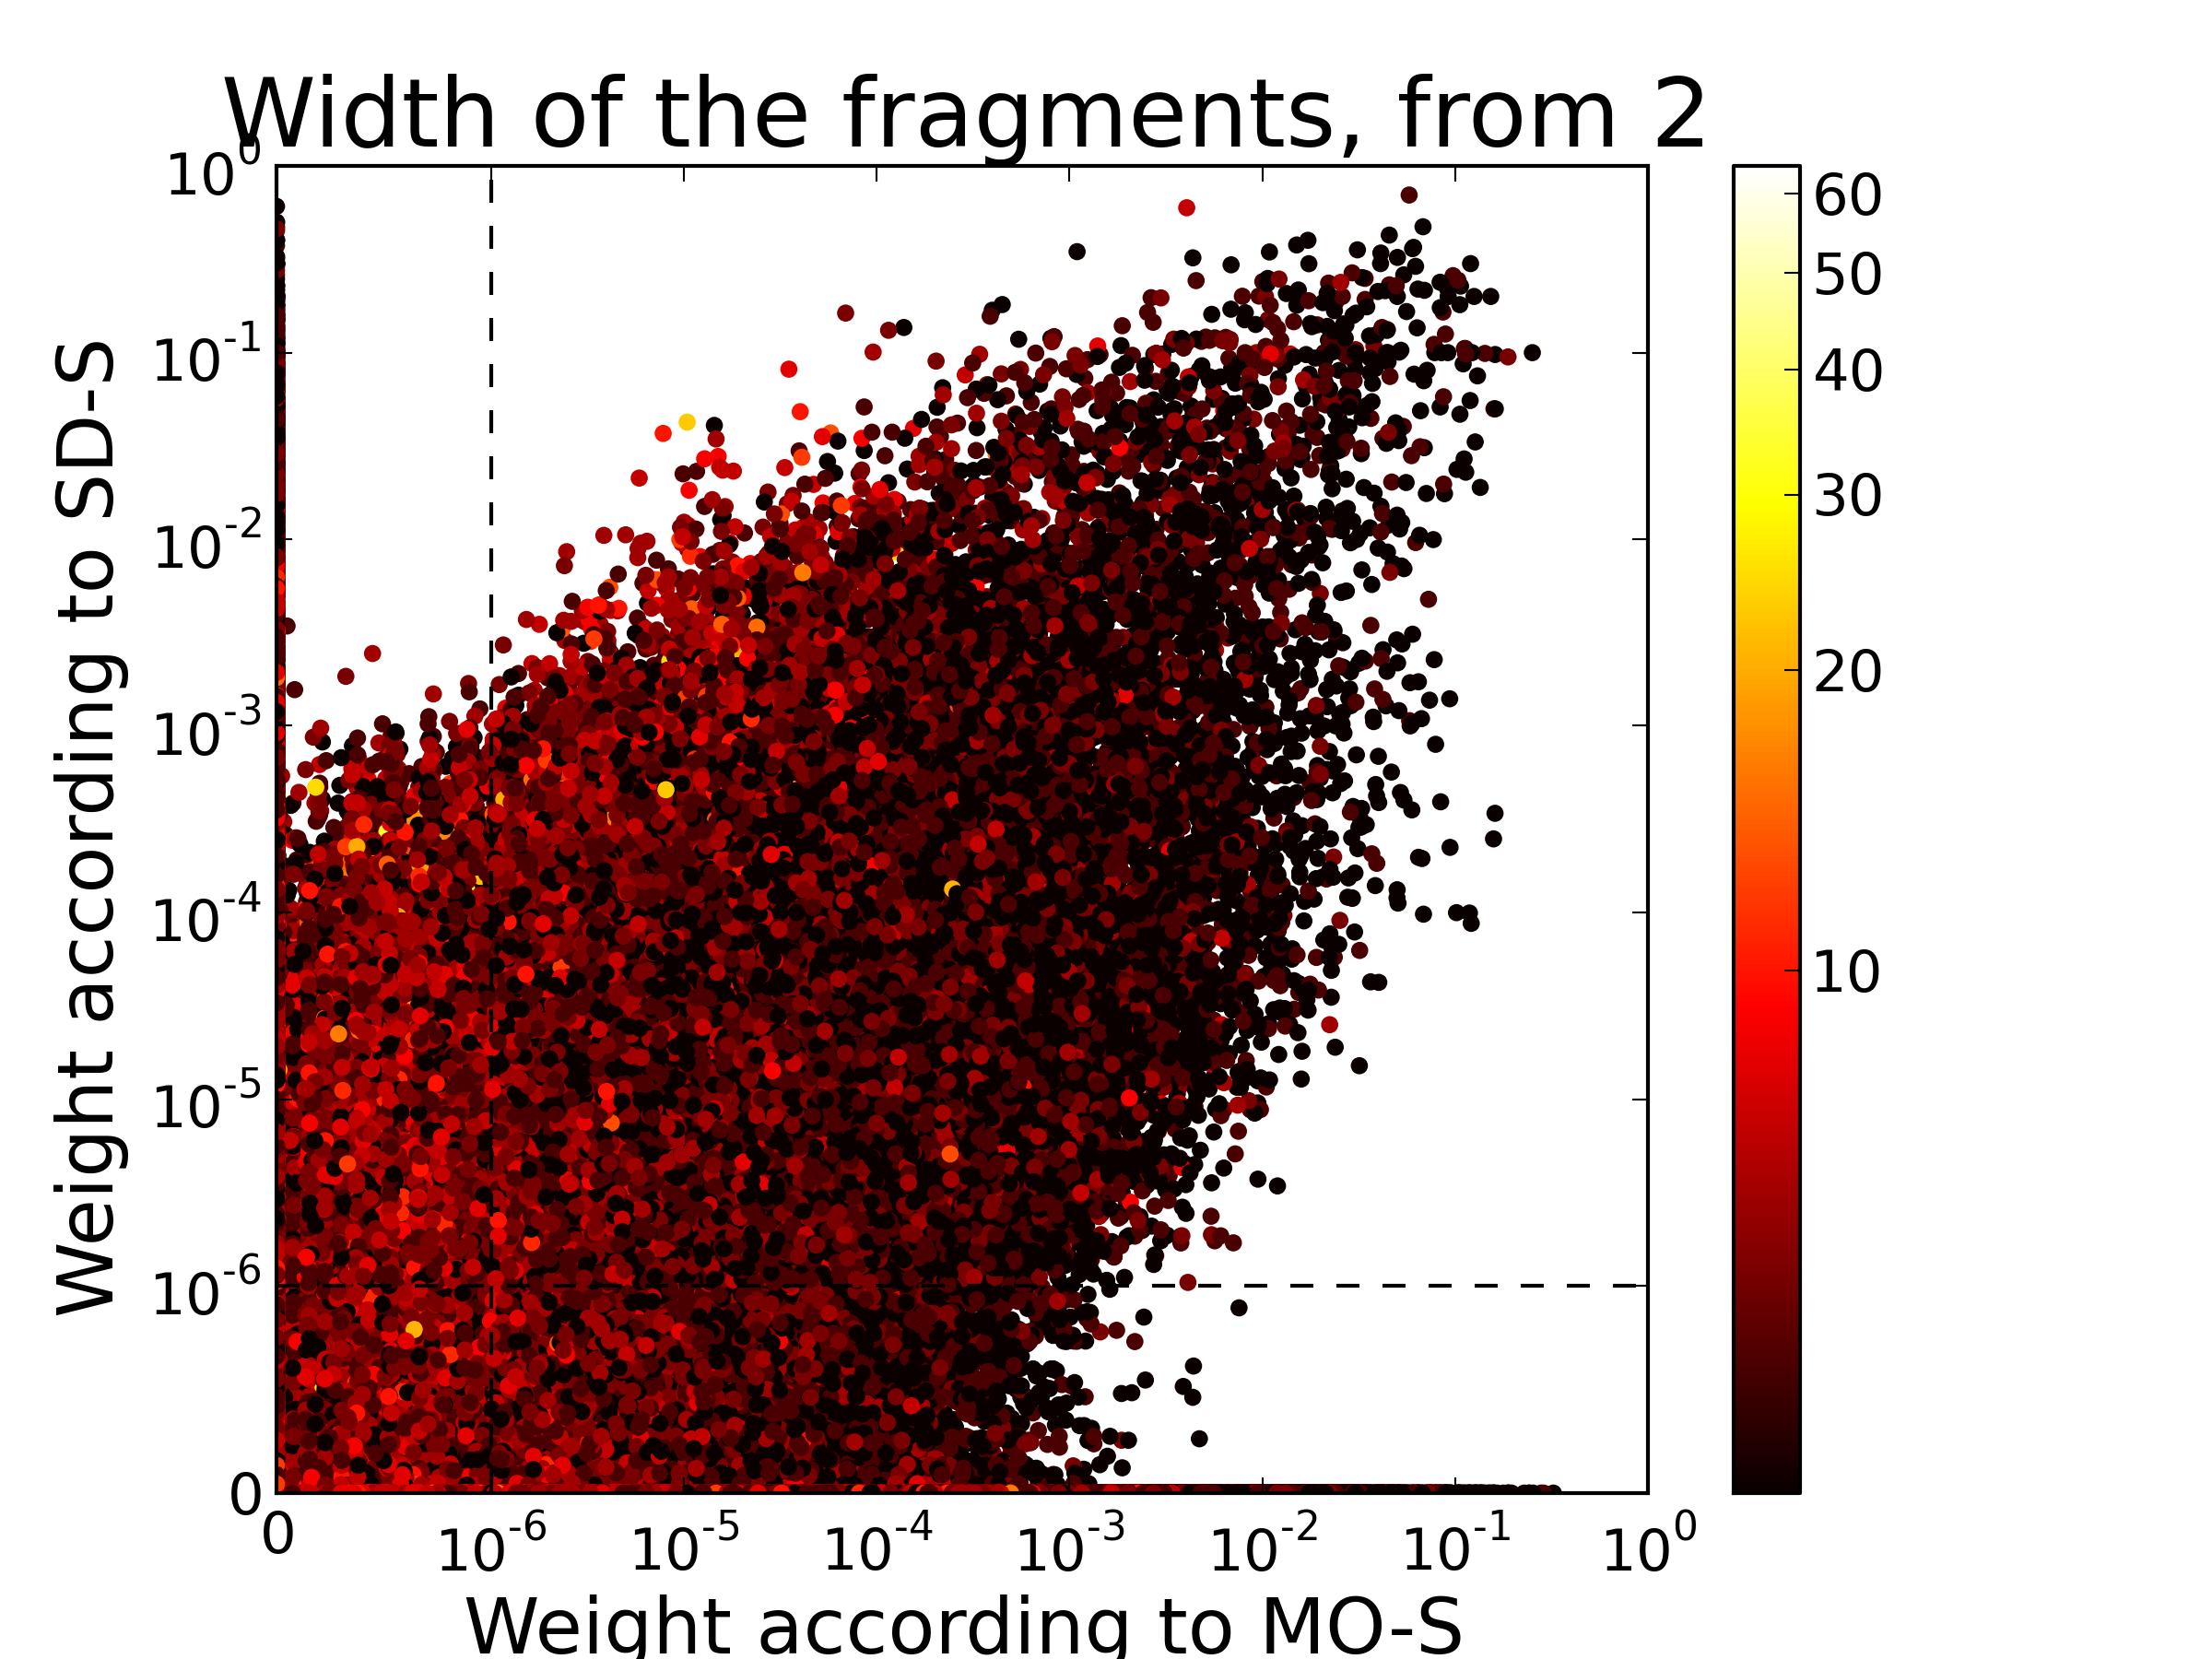
\includegraphics[width=\linewidth,trim=0.5cm 0cm 2.5cm 0.5cm, clip=true]{../data/plots/9.png}
\caption{Only fragments of depth 2 and deeper}
\label{f:width1b}
\end{subfigure}
\caption{Comparing shortest derivation to maximal overlap extraction by width of the fragments}
\label{f:width1}
\end{figure*}


%Diepe fragmenten zijn zwaarder in :
%	SD dan in MOS
%	SD dan MO
%	MO dan MOS (scherp)

%Brede fragmenten zijn zwaarder in:
% 	SD dan MOS (punt: CFG rules)
%	MO dan MOS (scherp)









%SDS MOS width


















